%! Date = 28/03/2023

% Preamble
\documentclass[a4paper,12pt]{article}

\usepackage[utf8]{inputenc}
\usepackage[T1]{fontenc}
\usepackage{lmodern}
\usepackage[english]{babel}
\usepackage{graphicx}
\usepackage[style=authoryear]{biblatex}
\usepackage{url}
\usepackage{hyperref}
\usepackage{booktabs}
\usepackage{tabularx}
\addbibresource{references.bib}

\begin{document}
    \begin{titlepage}
        \begin{center}
        {\huge\bfseries Suitability of an Internal Developer Portal to Support the Daily Work of BizDevOps Engineers\par}
            \vspace{2cm}

            {\scshape\large Certificate work in the \par}
            {\scshape\large CAS Digital Product Lead \par}
            \vspace{1cm}

            {\scshape\large HWZ University of Applied Sciences \par}
            {\scshape\large for Business Administration Zurich \par}
            \vspace{4cm}

            {\normalsize submitted to\par}
            \vspace{0.5cm}

            {\large Ralph Hutter\par}
            \vfill
            {\normalsize submitted by\par}
            \vspace{0.5cm}
            {\large Thierry Peng\par}
            \vspace{0.5cm}
            {\normalsize Address: placeholder 68, placeholder\par}
            {\normalsize  Place, Date: placeholder, \today\par}

        \end{center}
    \end{titlepage}


    \section*{Management Summary}
    %TODO
    \pagebreak


    \tableofcontents
    \pagebreak

    \section*{Used Tools}
    In addition to the sources mentioned in the bibliography\ref{sec:bibliograhpy}, the following aids and tools have been used
    \begin{itemize}
        \item Version control with Git and GitHub, the source code for this document is at \url{https://github.com/thpeng/mas/tree/master/src/mca-dpl23-1}
        \item Deepl at (\url{https://www.deepl.com/}) for supporting translations.
        \item Microsoft Forms for conducting a survey (\url{https://forms.office.com}) .
        \item The document has been written with \LaTeX  (\url{https://miktex.org/}) and using IntelliJ IDEA (\url{https://www.jetbrains.com/de-de/idea/})
    \end{itemize}

    \section*{Declaration of Honour}

    I hereby confirm that I have
    \begin{itemize}
        \item prepared the present thesis independently and without the use of sources or aids other than those indicated,
        \item identified the sources used as such, either verbatim or in terms of content,
        \item not yet submitted this work in the same or similar form to an examination board.
    \end{itemize}
    Bern, \today\newline
    \newline
    \newline
    \newline
    \begin{tabular}{@{}p{5.0cm}@{}}
        \hrulefill \\
        Thierry Peng
    \end{tabular}

    \pagebreak

    % max 15 - 20 pages beginning here


    \section{Introduction}
    \label{sec:introduction}
    SBB has an extensive and steadily growing IT landscape of applications and tools to support the digitization of the
    SBB's core business processes.
    These digitization efforts brought major changes to SBB's IT department.
    In less than ten years, the development model has changed from a pure waterfall to an agile methodology,
    cloud technologies were adopted while hardware-bound platforms were phased out, and a new internal organization was introduced,
    based on the separation of business and line management, has been introduced.
    Although these changes are now taking root and leading to various positive outcomes, they still pose a challenge
    due to the new and still existing complexity and the rapidly changing technological landscape.
    In addition, regulatory pressure has increased significantly in recent years, as exemplified by the
    HCBöV\footnote{Handbuch Cybersecurity für Betriebe des öffentlichen Vekehrs}, as well as the new Data Protection Act
    in Switzerland - nDSG.\linebreak
    Feedback from various employees in different roles from SBB's so called ``Digitalen Zone`` indicates, that the overall
    increase in complexity has an impact on the daily work of DevOps\footnote{DevOps is a combination of the words
    Development and Operations and can be either a role or a set of practices} engineers.
    The picture that is being painted is, although all information for the design, development and operation of
    applications is available in principle, it is maintained in very different places and forms.
    This makes the procurement of information for these activities time-consuming and requires that a DevOps
    engineer is already very familiar with the IT landscape of SBB .

    \subsection{Problem Statement and Controversy}
    \label{subsec:iproblemstatement}
    Research on the Internet about this problem, as well as guidance from vendors, indicates that there is greater momentum
    to address such issues with an internal developer portal (IDP). The central promise of the concept of an
    Internal Developer Portal is that it can reduce the so-called ``cognitive load`` of DevOps engineers by providing
    Processing and presenting information about teams, associated applications and their infrastructure usage.

    \subsection{Objective of the Certificate Work}
    \label{subsec:iobjective}
    The aim of this certificate thesis is to investigate whether and to what extent the above-mentioned problem
    can be solved by the introduction of an internal developer portal.
    In a first step, the benefits of the concept of an internal developer platform are elaborated and placed in the
    into the general context of software development and the operation of IT systems in the SBB.
    In a second step, the problem of complexity and lack of integration is underpinned with a quantitative survey.
    The third part consists of bringing together the results of the survey and the value proposition and making a
    recommendation for action.


    \section{Value Proposition for an Internal Developer Portal}
    \label{sec:vp}
    An Internal Developer Portal is a web-based information catalogue which is tailored for the needs of
    engineers operating IT systems, developing software and other related work.
    Internal Developer Portal are proposed as the solution for perceived problems\parencite{backstagestory} of DevOps
    engineers while developing and operating IT Systems such as
    \begin{itemize}
        \item A lack of a central repository for reliable and tailored information
        \item A high cognitive load of engineers because of switching between multiple and very different tools while developing or operating IT Systems
        \item Increasing the developer experience by abstracting away complexity in infrastructure management
    \end{itemize}
    One potential source of information for using in the Internal Developer Portal is an Internal Developer Platform.

    \subsection{Internal Developer Platform}
    \label{subsec:vpplatform}
    Gartner makes a differentiation between the concept of an Internal Developer Portal and an Internal Developer Platform:
    ``internal developer portals serve as the interface through which developers can discover and
    access internal developer platform capabilities``\parencite{gartner} .
    An Internal Developer Platform (Platform), according to the COO Christoph C. Richter from Humanitec\parencite{richteretal} ,
    should consist at least of the following component:
    \begin{itemize}
        \item Application Configuration Management
        \item Infrastructure Orchestration
        \item Environment Management
        \item Deployment Management
        \item Role-Based Access Control
    \end{itemize}
    In some other sources, there are also additional components mentioned, e.g. Observability\parencite{xenon}.
    XENONSTACK as well as Humanitec mentioned before, are suppliers of Internal Developer Platform solutions with
    different capabilities.
    The capabilities and components of Internal Developer Platforms are not unique to the products of those two suppliers.
    In most contemporary IT operations or software development departments these components and practices are well-known
    and used widely.
    Beyond the size of a very small team, it is necessary to use tooling to know where, in which version and with what
    configuration a software artifact was installed.
    The reason behind this may be to coordinate a new software rollout, test the software on a dedicated stage, fix bugs
    or develop new features and to solve incidents caused by your software.
    Thus, it can be argued, that the concept of an Internal Developer Platform is not unique to specific products
    or offerings, but can be used on a set of tooling and practices supporting IT operations and software development.
    This set of tooling and practices can be viewed as predecessors of Internal Developer Platforms and are usually
    distinct solutions or products.
    For example there is a separate Configuration Management Database
    to address the need of Application Configuration Management or there is a purpose built Continuous Integration /
    Continuous Deployment pipeline for addressing the need for a Deployment Management.
    These solutions are not necessarily integrated with each other.
    It may be also the case, that these
    products or solutions were established before the advent of Agile Methodologies and DevOps.

    \subsection{DevOps}
    \label{subsec:devops}
    With DevOps, the traditional disciplines of IT operations and software development are much more integrated to
    to reduce friction, release features more frequently, and improve product quality\parencite{safedevops}.
    Prior to DevOps, it was common to use different tools and processes for the development and operations roles
    because these two roles were housed in different departments or teams.
    There is a fundamental trade-off in developing and operating solutions separately.
    Developers are measured on responsiveness and speed of delivery.
    Operators, on the other hand, are measured by the secure and stable operation of solutions.
    One of the basic principles of DevOps was coined by Werner Vogels, the current CTO of Amazon;
    ``You build it, you run it``\parencite{vogels}.
    This means that the same team that develops the software also runs it.
    With DevOps, a team takes full responsibility over the lifecycle of a software or platform.
    In combination with agile methodologies such as Scrum\footnote{Scrum is an iterative software development methodology}
    or SAFe\footnote{SAFe stands for Scaled Agile Framework and adds orchestration layers above agile (Scrum) teams for
    a better cross-team and product-centric alignment}, business-oriented individuals are also integrated into this
    cross-functional team.
    An example of a business-oriented role in a DevOps team is the Product Owner\parencite{safepo}.
    This also means that a team must have a wide range of skills and access to various tools needed for their work.
    Such tools can be used for activities such as requirements engineering, solution architecture, software development
    but also anything needed to operate the software.
    Especially the operation of the software is a tool-intensive work.
    There are tools for logging, monitoring, incident handling and alerting.
    In the event of an incident, a configuration management database or an enterprise architecture database are critical
    to find out who a particular application or resource belongs to.
    This information is important to determine the root cause and quickly resolve the incident.
    Although DevOps offers numerous benefits, it is quite complex for a team member in an agile and DevOps team.
    Here, the Integrated Developer Portal offers several suggestions to help individuals and teams with their day-to-day operations.

    \subsection{Internal Developer Portal}
    \label{subsec:vpportal}
    Manjunath Bhat from Gartner argues, that an Internal Developer Portal has three main characteristics\parencite{gartner}:
    \begin{itemize}
        \item Abstraction
        \item Developer-centric view
        \item Pluggable framework
    \end{itemize}
    The overarching goal of these characteristics are to increase the devops experience by shortening the time searching
    and interpreting information.
    The search task is supported by a central software catalogue.
    The interpretation of the data is supported by an underlying logical model, which describes the assets, technologies
    and their relationship in between.
    The logical model is different between each of the internal developer portal but have some common elements.

    \subsubsection{Vendors and Products}
    \label{sssec:vendors}
    While it's not the focus of this certificate work to delve into the details of each possible product on the market
    and make a comparison between them, it's worthwhile to describe a few.
    Redpoints mentions five products as ``Universal Service Catalogue`` offerings\parencite{devportalsprimer}.
    This kind of Internal Developer Portal is not tied into specific cloud offerings such as AWS, Azure or Google
    Cloud Platform (``API Catalog tied to an API Gateway / Service Mesh``)and has no opinion about a particular application
    architectural style, such as the products mentioned in the category ``Microservice Catalog``.
    \begin{table}[!htbp]
        \begin{center}
            \begin{tabularx}{\textwidth}{lllll}
                \toprule
                Vendor   & Product      & Year & License               & Deployment  \\
                \midrule
                Spotify  & backstage.io & 2020 & open source           & self-hosted \\
                Lyft     & clutch.sh    & 2020 & open source           & self-hosted \\
                Moment   & moment.dev   & Beta & proprietary           & SaaS        \\
                Opslevel & opslevel.com & 2018 & partially open source & SaaS        \\
                \bottomrule
            \end{tabularx}
            \caption{\label{tab:vendors} Vendor and Products.}
        \end{center}
    \end{table}
    Roadie is omitted from the table \ref{tab:vendors} because it's a commercial offering of Backstage.
    It seems, there are two main directions; Backstage and Clutch have been developed by two big tech companies for their
    internal audience, have been made available as opensource and Moment
    and OpsLevel are purposefully built by startups as a product and have commercial offerings.
    For the further discussion about the value proposition of an Internal Developer Portal, some screenshots and concepts will
    be used from Backstage.
    Backstage has been built by Spotify, which invests heavily in what they call the
    ``developer experience`` (DX)\parencite{spotifydx}.
    Additionally, Backstage was adopted in 2020 as an incubating project into the Cloud Native Computing Foundation\parencite{cncf} .

    \subsubsection{Discoverability and Information Gathering}
    \label{sssec:disc}
    The Software Catalogue is the main feature of an Internal Developer Portal.
    Its purpose is to make the capabilities of the Internal Developer Platform accessible for an engineer as seen in the
    screenshot in figure \ref{fig:catalog}.

    \begin{figure}
        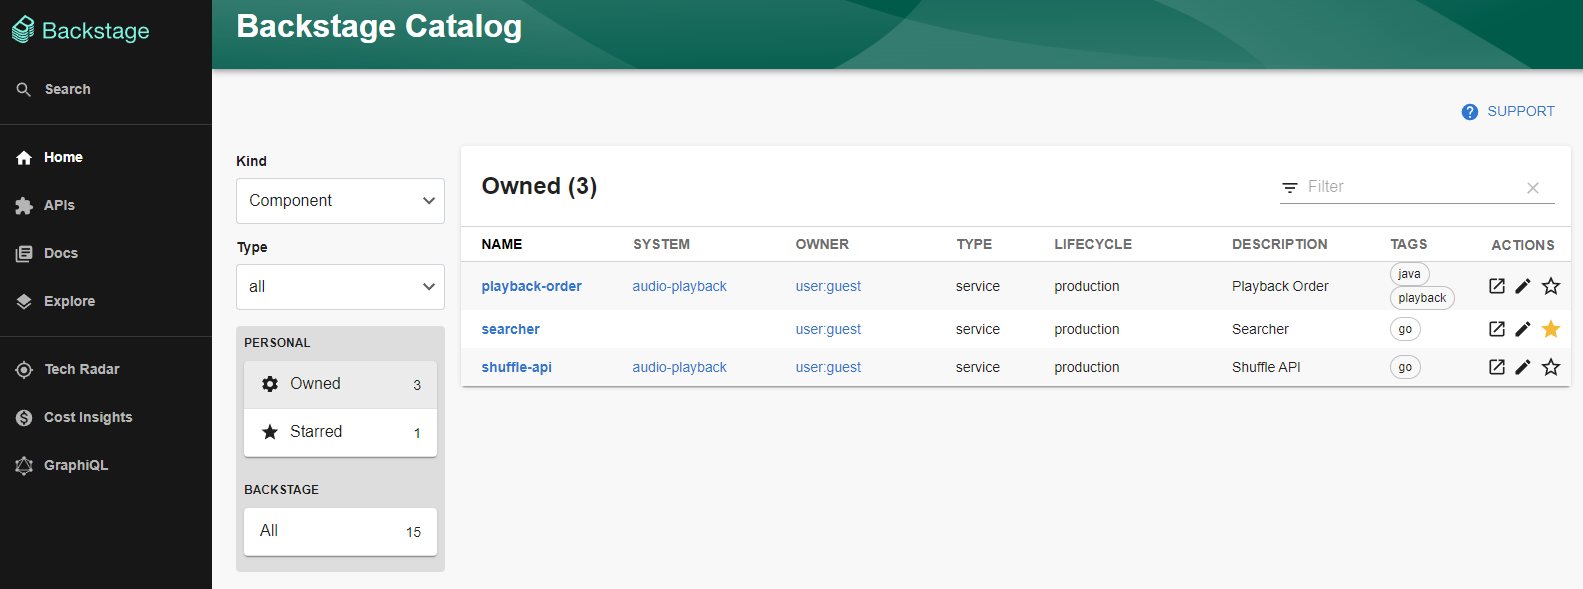
\includegraphics[width=\linewidth]{backstage_catalog}
        \caption{The Software Catalog from the Backstage Demo\parencite{backstagedemo}}
        \label{fig:catalog}
    \end{figure}
    Its content may be any combination of
    \begin{itemize}
        \item Teams with members
        \item Applications
        \item Infrastructure and platforms
        \item Most importantly, the relationships between those. These attributes are modelled, e.g. an application is owned by a team.
    \end{itemize}
    Data may be shown in a tabular fashion or may be shown as a relationship graph and the catalogue is searchable.
    An Engineer may bookmark its favourite items and its own resources are marked by ``owned``.

    In addition to the catalogue with its tabular overview, there is a details view seen in figure \ref{fig:portaldetails}.
    \begin{figure}
        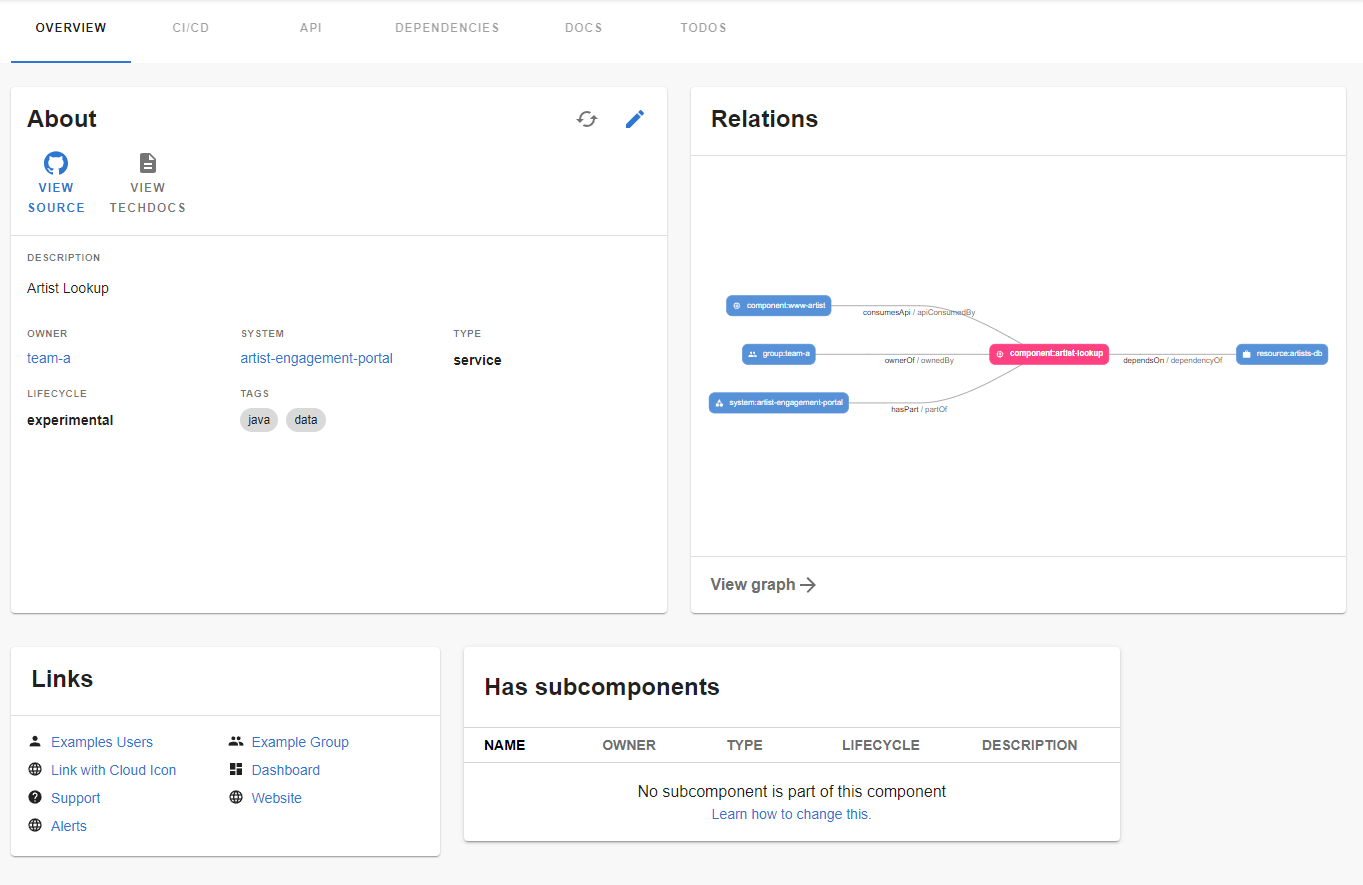
\includegraphics[width=\linewidth]{backstage_item_details}
        \caption{Details about an artifact}
        \label{fig:portaldetails}
    \end{figure}
    In the details view more attributes are shown for the chosen item from the overview.
    Depending on the kind of item, different attributes are shown.
    For an application, it may be its used resources, consumed and provided APIs and other subcomponents.
    For teams, the members are shown and its owned resources and its contact details.

    % not sure if to include this section in the final document.

    \subsubsection{Platform as a Product}
    \label{sssec:paap}
    In some implementations of an Internal Developer Portal, the catalog is not just a copy of an architecture database.
    In addition to the aforementioned applications, platforms, organizational data, and resources, other products of the
    of the teams are represented.
    For example, platform teams may provide support and consulting for their platform or area of expertise and offer this service.
    Some teams use the Internal Developer Platform to showcase code or libraries to create an inner-source community.
    In an expertise-sharing session between SBB and Booking.com, Booking.com reported its Internal Developer Portal as a
    standalone product that is managed by a dedicated team.
    This team is also responsible for onboarding other platform and application teams, convincing them of the
    value of an integrated Internal Developer Portal.

    \subsubsection{Golden Path}
    \label{sssec:goldenpath}
    The term ``Golden Path`` was coined by Spotify\parencite{spotifygoldenpath} and is itself a reference to the Frank
    Herbert`s Dune trilogy and describes the only viable way to do things right.
    A Golden Path is a ready-to-use template for getting a project started quickly.
    It can consist of software engineering artifacts and preconfigured infrastructure components and is usually very
    opinionated.
    Opinionated means that the context of the enterprise is already considered, such as internal regulations,
    the currently supported tech stack, and other internal specifics.
    For example, a golden path for a database is already built into the company's security infrastructure,
    Logging is ensured, and some best practices for database configuration and modeling are implemented.
    Golden Paths are not necessarily product-specific; they can encompass a typical development stack used in the enterprise
    used in the enterprise, such as a Golden Path for a web application.
    This stack may consists of a frontend built
    with Javascript, a Java backend and an Oracle database, all integrated into a single build pipeline for CI/CD\footnote{CI/CD stands for continuous
    integration and continuous deployment and is a practice in software engineering. Its main focus is to automate all steps
    between development and rolling out on production, such as quality assurance, building artifacts and installing them.},
    securely configured and with the enterprise look and feel already established.
    With such a template mechanism, new applications can be built faster, the same solutions can be reused for overarching
    reused, and developers don't have to write tedious code to integrate each of these components with each other.
    each other.

    \subsubsection{Technical Documentation}
    \label{sssec:techdoc}
    Platforms that use an Internal Developer Portal may choose to migrate their user-facing documentation to the portal.
    The basis for this technical documentation can be a solution based on Markdown\parencite{backstagetechdocs}
    or a similar syntax.
    The advantage of this approach is that the documentation is treated like code and can be integrated into the same toolchain.
    For example, the documentation sits alongside the platform automation code, is peer reviewed, created
    and published in sync with the platform's update cycle.
    In the discussion mentioned in the chapter \ref{sssec:paap}, Booking.com talked about an integration in their Internal
    developer Portal, where communication about lifecycle and changes to their platforms is integrated into their portal.

    \subsubsection{Visibility of Expertise}
    \label{sssec:expertise}
    Splunk\footnote{Splunk is a company specialised in creating software for loganalysis and monitoring and it is known
    for its product with the same name}
    describes a use case, how to leverage an Internal Developer Portal to make expertise visible in their
    company\parencite{splunkidp} .
    Their solution is to enrich teams and users with additional data about their knowledge and let other user give feedback
    how a team or user did support them, called a ``Bravo`` in their terminology.
    Thus, they create something like a social network inside their company for connecting people to solve problems or
    easing the way how to find people with specific skills or knowledge.

    \subsubsection{Extendability of the Platform}
    \label{sssec:extendability}
    As shown in chapter\ref{sssec:vendors} , there are multiple offerings of Internal Developer Portal and varying
    implementations.
    In case of the Software-as-a-service offerings, the extendability consists of using plugins for well-known
    technologies or products and preparing and inserting the companies data for the catalogue feature.
    The self-hosted variants, such as Backstage and Clutch are more like a skeleton or a framework.
    For both products, there are pre-built binaries which are installable and runnable, but you can choose to build your
    own Internal Developer Portal and use these products as a starting point.
    Both support custom-made plugins on the front-end side which may use additional datasource outside the direct
    internal developer portal.
    This approach is handy for decentralized organisational forms where each team have maximal autonomy about how they
    reach their goals, but would like to use and contribute to a centralized catalogue by adding data and functionality
    via plugins.
    The plugin architecture allows to leverage your Internal Developer Portal with the tooling landscape in a
    single and integrated user experience for DevOps Engineers.

    \subsubsection{FinOps}
    \label{sssec:finops}
    FinOps is a practice to enable DevOps Teams to make decisions about resource usage and creates transparency
    about the costs incurred by these decision.
    The FinOps foundation defines\parencite{finopsdefinition} this practice as ``FinOps is an evolving cloud financial management discipline and
    cultural practice that enables organizations to get maximum business value by helping engineering, finance,
    technology and business teams to collaborate on data-driven spending decisions.``.
    An Internal Developer Portal may help with this practice by providing functionality for one of the basic discipline
    FinOps: ``Understanding Cloud Usage And Cost``.
    The Backstage.io Demo shows one possible implementation in the Demo\parencite{backstagedemocost}.
    This capability enables a DevOps team to take responsibility also in the financial domain and creates transparency
    for the business what the true costs of their product is.


    \section{Situation at the SBB IT}
    \label{sec:sbbit}
    The IT department of the Swiss Federal Railways (SBB) consists of around 1300 specialists and is responsible for
    700 applications\parencite{sbbitkennzahlen}.
    The applications built and operated by this department are used for a wide range of use cases.
    For example, some applications are covering generic enterprise use cases such as human resource management, finance
    and controlling.
    Other software is specially built for mission-critical, day-to-day operations of the railway such as the Rail Control
    System (RCS)\parencite{sbbrcs} .
    An SBB IT application may be a purchased product, may be developed in-house or is a combination thereof which is
    sometimes called a ``customization``.
    Applications and products, built and operated by the SBB, are regulated by different standards and regulations of the
    swiss government or by industry initiatives.
    Examples are the EN 50128 standard by the European Committee for Electrotechnical Standardization (CENELEC)\parencite{cenelec},
    which governs among other things the development of safety-related software with different requirement levels
    or the HCBöV\parencite{hcboev} with regulations concerning cyber-security, risk management, business continuity
    management among others.
    In addition to the more business-oriented applications, there is a need for platforms and tools to help create
    and operate these.
    Examples are a PaaS\footnote{A platform-as-a-service (PaaS) is a platform which exposes resources such as compute or
    storage to applications. The team which is building an application is relieved from the burden of obtaining and
    provisioning resources on a hardware level. A well-known implementation of a PaaS is Kubernetes from the CNCF.},
    databases, messaging but also networking, monitoring, security and
    speciality services like UX or test-engineering and others.

    \subsection{Internal Developer Platform}
    \label{subsec:sbbplatform}
    The SBB IT has for most of the core components of an Internal Developer Platform, as laid out in chapter\ref{subsec:vpplatform},
    already solutions in place:
    \begin{itemize}
        \item Application Configuration Management - is centered around the practice of GitOps\parencite{hashicorpvault}
        \item Infrastructure Orchestration - for example, SBB uses OpenShift since 2015\parencite{rhsbbopenshift}
        \item Environment Management - provided by OpenShift and CI/CD Pipelines
        \item Deployment Management - is provided by CI/CD pipelines built on Tekton and ArgoCD\parencite{sbbtekton}
        \item Role-Based Access Control - built-in in most of the SBB IT platforms
    \end{itemize}
    In addition, there are several other tools and applications used for the day-to-day operations and development.
    Most notable are the following
    \begin{itemize}
        \item Development and operation are dependent on a Wiki Software for documentation and communication.
        \item An Enterprise Architecture Database contains the information about used technologies, platforms and
        dependencies, as modelled by the architects
        \item An IT Service Management Platform contains the data concerning team contact information and support groups for applications
        \item A Configuration Management Database contains data about used assets, resources and relations to applications
    \end{itemize}
    Thus, it could be argued, that the foundation for an Internal Developer Platform is in place, but there are two
    critical pieces missing.
    First, most of the components mentioned are only partially integrated with each other.
    Examples for missing integration are different identifier for assets, unaligned authorization such as per-user vs.
    per-group models and manual data maintenance.
    Second, there is no central view to aggregate data contained in these applications and tools for the benefit of
    the DevOps engineers.

    \subsection{DevOps}
    \label{subsec:sbbdevops}
    In 2015 the practice of DevOps and a PaaS was first introduced in the SBB IT .
    The stated goals of these additions was to solve the rising complexity in operations and the perceived low velocity
    in responding to change\parencite{sbbdevops} .
    Four years later, a reorganisation brought a new operating model to the SBB IT, based on agile principles, DevOps and SAFe
    and created the role of the BizDevOps engineer\parencite{sbbagile} .
    Most of the roles from before the restructuring, such as application engineer, operations manager, test engineer, or requirements engineer
    have been transformed into this BizDevOps engineer role.
    Even some formerly business-oriented roles are now called BizDevOps engineers and are integrated into these cross-functional
    teams.
    DevOps teams in 2023 are now the established standard, but they are still working mostly with tools for developing and
    operating from the organization before.
    The tools themselves may be state of the art in their fields, but they were not purchased or developed with
    end-to-end integration in mind that would benefit a BizDevOps engineer.

    \subsection{Internal Developer Portal}
    \label{subsec:sbbportal}
    Most BizDevOps teams of the SBB help themselves with some kind of organization for the necessary information
    for the day-to-day work.
    A common approach is to leverage the internal Wiki software, where each teams maintain their relevant http link
    collection in the context of their project in one or more pages.
    When someone joins a team, its first task is in most cases, that he/she must familiarize himself/herself with this
    collection.
    Naturally, these link collection grow outdated and its maintenance needs also effort from a team.
    If whole teams are being staffed, for example with models such as managed capacity or near-shore, it is even worse
    for getting up to speed.
    While this problem about discovery and sharing knowledge isn't fully addressed, there were some efforts to create
    a self-service portal for ordering resources.
    The reason for this portal was, that platform teams weren't happy with unstructured ordering with email, telephone or
    others ad-hoc methods and built a modular and decentralized portal for this use case.
    However, there was no single owner of the portal and after the immediate pain point of the platform has been adressed,
    there was no further effort to expand the functionality until now.


    \section{Method}
    \label{sec:method}
    The method chosen to verify the observations about the state of the DevOps Experience and to evaluate the value proposition
    of an Internal Developer Portal, is to hold a survey.
    The survey is created with a customer journey based on different BizDevOps personas.
    The personas and the customer journey are based on a preliminary, internal work\parencite{sbbjobstobedone}.

    \subsection{Customer Journey}
    \label{subsec:cusjour}
    The customer journey is focused on the interaction of different personas with the existing Internal Developer Platform.
    The assumption is, that this interaction between the BizDevOps Engineers and the Internal Developer Platform has a big
    impact on the DevOps Experience.
    The personas of the customer journey are roles which are quite common in a BizDevOps team in the SBB IT.\\
    \textit{Peter Plattform} is working as a platform engineer and interested in the lifecycle of resources and platforms which
    are necessary for the building and operating of application in his team.\\
    \textit{Diego Developer} is a software engineer and his duty is to work on features and enabler in the context of his team.
    He is interested in building solutions and needs know-how and best practices for doing so.
    His secondary interest is, to get his work as fast as possible and with the highest quality into the production environment.
    \textit{Norbert Neuling} is the rookie in the team.\\
    He wants to acquire knowledge, try out the established technologies or platforms and needs a solid template for creating
    his own solutions.\\
    \textit{Agnes Architekt} is working as an IT architect.
    The product owner of the team asked her to identify variants to lower the operation cost.
    She is also very interested
    to know about changes in the platforms, so that she can inform the product owner and put the necessary enablers in
    the next product increment\footnote{SAFe terminology for a cycle of usually five two-week SCRUM Sprints of agile software development.}.\\
    \textit{Ida Incident} is working on an operational issue.
    She needs to know the technical topology of her application and the used platforms.
    She has to know, which team is responsible for which platform and how she could reach them.\\
    For more information, see figure\ref{fig:customerjourney}

    \subsection{Quantitative Survey}
    \label{subsec:quansur}
    For a quantitative survey, a mix of questions were created based on the customer journey.
    Some are related to the value proposition of an Internal Developer Portal and some questions about other known or
    suspected issues around the existing Internal Developer Platform.
    The survey is intentionally kept short.
    The expectation is, that a short survey generates more responses because for the respondent it is only a small time investment.
    The intended target of the audience are the BizDevOps engineers of the SBB.
    One of the main information source for the BizDevOps engineers is the CLEW\footnote{CLEW stands for Cloud, ESTA,
        itself an acronym of Entwicklungstack and WZU, Werkzeugunterstützung} blog.
    This blog has an audience of 780 subscribers.
    The survey itself is built with Microsoft Forms.
    The start date of the survey was the 24.04.2023 and the end date was on 08.05.2024.

    \subsubsection{Questions}
    From the sixteen steps in the customer journey seventeen rating questions were created.
    The rating questions are documented in the appendix in table \ref{tab:ratingquestionstable}.
    The relation between the value proposal in chapter \ref{sec:vp} and the questions are as follow:
    \begin{itemize}
        \item Questions 1, 13 and 14 relate to Discoverability and Information Gathering in chapter \ref{sssec:disc}
        \item Question 2 relates to Visibility of Expertise from chapter \ref{sssec:expertise}
        \item Questions 3 and 17 relate to Technical Documentation, chapter \ref{sssec:techdoc}
        \item Question 10 relates to the chapter \ref{sssec:goldenpath}, Golden Path
        \item Question 12 relates to FinOps, chapter \ref{sssec:finops}
    \end{itemize}
    Questions 4, 11 and 16 do not have a strong correlation with the concept of an Internal Developer Portal.
    However, these three questions relate to the capabilities of the existing Internal Developer Platform.
    The questions 5, 6, 7, 8 and 9 gauge the maturity of the Internal Developer Platform concerning the lifecycle of resources.
    The may be integrated in a Internal Developer Portal because of its Extendability described in chapter \ref{sssec:extendability}.
    However, information about integrating these use cases in an Internal Developer Portal are scarce.
    There are no direct questions about the chapter Extendability \ref{sssec:extendability} and Platform as a Product
    \ref{sssec:paap}.
    Extendability is more of a non-functional requirement for the choosing of the concrete Internal Developer Portal
    solution instead of a wanted feature for a user of this portal.
    Platform as a Product is more a goal for the SBB IT internal product management to make the Work of the BizDevOps
    teams more visible and accessible and are not an intrinsic goal of an engineer.
    Question 15 ask a question about support in the incident process and is neither related to an Internal Developer Platform
    nor an Internal Developer Portal. \\
    The survey and the questions are scoped on the DevOps experience and usage of the platform, products or services of
    the so called Core\footnote{Core consists of multiple DSRVs, most with mission-critical platforms} DSRVs\footnote{
        A DSRV stands for Digital Service and is one or more teams with multiple services and platforms. A DSRV is built
        around a domain, eg. Monitoring,        Cloud infrastructure, PaaS and others}.
    It is not necessary, that the respondent must have used all of these services.
    The scope is also usage in the last three months.
    The rating questions have choices from one to five star and are mandatory.
    The description of the meaning of the rating is given as follows
    \begin{itemize}
        \item One star - non-existent or unknown
        \item Two star - with room for improvement
        \item Three star - I can work with it, corresponds to what I expect
        \item Four star - above average
        \item Five star - super, that's what makes you
    \end{itemize}

    In addition, two more questions, documented in table \ref{tab:oetable} were asked for gathering additional data for
    internal needs of the SBB IT.
    One question has a free text answer to solicit more input and to generate additional interview partner
    for a qualitative survey.
    This question is optional for the respondent.
    These interviews and the resulting insights are not part of this certificate work.
    The final question\footnote{The final engagement question was added based on input of the internal product management team}
    is a engagement questions and tries to gauge the overall satisfaction of the BizDevOps engineers
    with the available services and platforms of the so called Core DSRVs.
    % 2.3.2 Discoverability -> 1, 13, 14 (strong)
    %2.3.3 Platform as a Product n/a
    %2.3.4 Golden Path -> 10 (strong)
    %2.3.5 Technical Documentation, -> 3,17 -> ev. noch Extend! (strong)
    %2.3.6 Expertise -> 2, (strong)
    %2.3.7 Extendability
    %2.3.8 FinOps -> Frage 12. (strong)
    % n/a -> 4, 11, 16 (platform)
    % Lifecycle: -> 5, 6, 7, 8, 9 (weak)
    % monitoring, -> 15 (none)

    \subsubsection{Result of the Rating Questions}
    \label{sssec:rratque}
    In the two weeks run time of the survey, the response rate was 9.74\% with 76 respondents.
    Based on a confidence level of 95\% the margin of error is 10\% for this survey.
    The raw results for the rating questions are included in table \ref{tab:rawratingquestionresultstable}.
    The calculated values for the rating questions are present in \ref{tab:ratingquestionresultstable}.
    Overall, the seventeen question have an average of 3.40, the average of detractors is 18.5\% of the
    respondents and the average of the promoters is 51.3.
    An aggregated result for the five value proposals with eight related questions are documented in the table \ref{tab:aggregateidpresults}.
    \begin{table}[!htbp]
        \begin{center}
            \begin{tabularx}{\textwidth}{llllll}
                \toprule
                Theme           & Ids       & Average & Detractors & Promoters & Variance \\
                \midrule
                Discoverability & 1, 13, 14 & 3.11    & 24.4\%     & 35.1\%    & 0.826    \\
                Expertise       & 2         & 3.64    & 12.0\%     & 65.3\%    & 1.097    \\
                Documentation   & 3, 17     & 3.41    & 18.7\%     & 51.9\%    & 1.056    \\
                Golden Path     & 10        & 3.21    & 20.0\%     & 42.7\%    & 0.850    \\
                FinOps          & 12        & 2.62    & 45.3\%     & 21.3\%    & 1.420    \\
                \bottomrule
            \end{tabularx}
        \end{center}
        \caption{\label{tab:aggregateidpresults} Aggregated results for IDP related questions.}
    \end{table}

    In contrast, the aggregated result of the questions about other topics, grouped by questi§ons about lifecycle of resources,
    generic Internal Developer Platform questions and about Incident handling are as seen in table \ref{tab:nonidpresults}.

    \begin{table}[!htbp]
        \begin{center}
            \begin{tabularx}{\textwidth}{llllll}
                \toprule
                Theme     & Ids           & Average & Detractors & Promoters & Variance \\
                \midrule
                Lifecycle & 5, 6, 7, 8, 9 & 3.59    & 13.9\%     & 59.5\%    & 1.147    \\
                Platform  & 4, 11, 16     & 3.46    & 15.6\%     & 54.7\%    & 1.025    \\
                Incident  & 15            & 3.92    & 10.7\%     & 74.7\%    & 1.099    \\
                \bottomrule
            \end{tabularx}
        \end{center}
        \caption{\label{tab:nonidpresults} Aggregated results for non-IDP related questions.}
    \end{table}

    \subsubsection{Result of the Open Question}
    \label{sssec:ropque}

    % techdoc + Benach: IIIIII
    % CI/CD kritik: IIII
    % Enhancement local installation: III
    % Discovery: IIII
    % thanks: III
    % finOps: II
    % infrastructure-as-code missing: II
    % critic of vision: II
    % missing consultancy / unified support: II
    % gandalf kritik: II
    % multiple tools for the same job: I
    % Availability of toolchainL: I
    % non-informatiker: I
    % missing review/freigabeprozess: I
    % missing resource lifecycle for delete, upgrade: I
    % missing devsecops: I

    \subsubsection{Result of the Engagement Question}
    \label{sssec:rengque}


    \section{Conclusion}
    \label{sec:conclusion}
    \pagebreak
    % max 15 - 20 pages end here


    \section{List of Sources}
    \label{sec:bibliograhpy}
    \printbibliography[heading=none]


    \section{Appendix}
    \label{sec:appendix}

    \subsection{Customer Journey Map}
    \label{subsec:cusjourmap}
    \begin{figure}
        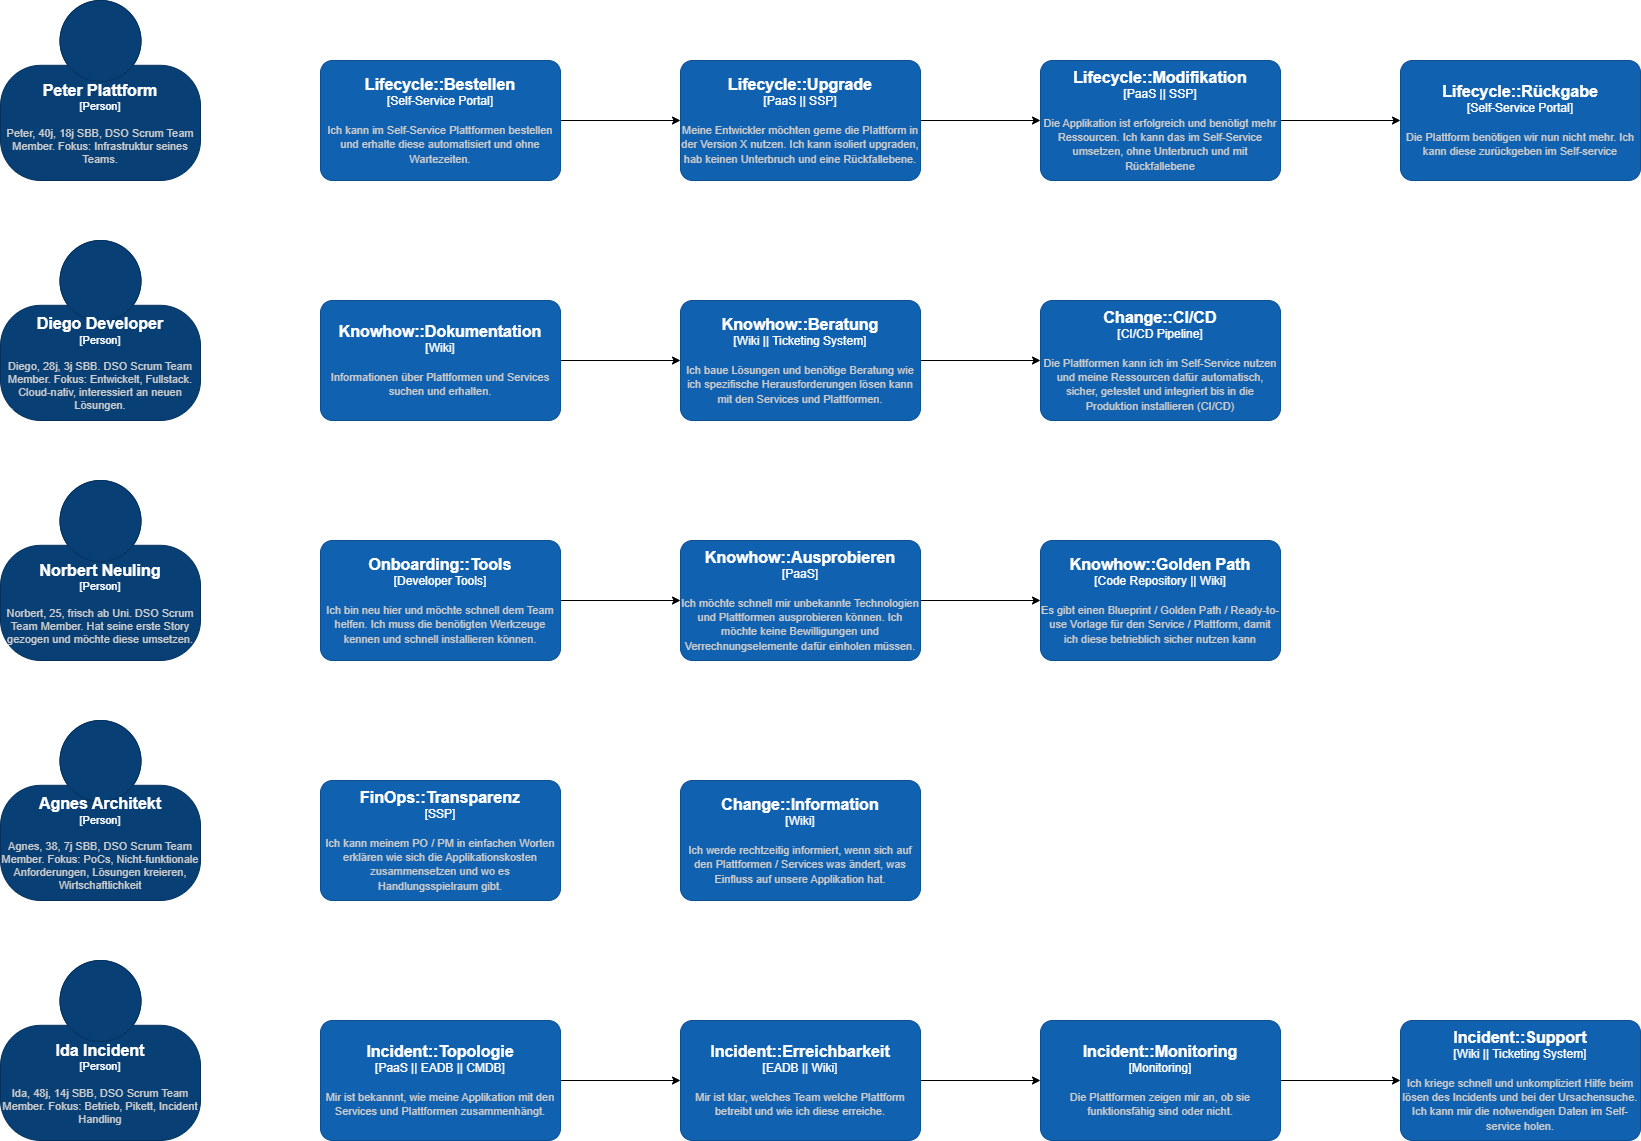
\includegraphics[angle=270,origin=c,width=\linewidth]{customer-journey.png}
        \caption{Customer Journey Map}
        \label{fig:customerjourney}
    \end{figure}

    \subsection{Survey}
    \label{subsec:survey}

    \subsection{Rating Questions}
    \label{subsec:rating}
    \begin{table}[!htbp]
        \begin{center}
            \begin{tabularx}{\textwidth}{lX}
                \toprule
                Id & Question                                                                                                                                                                              \\
                \midrule
                1  & Auffindbarkeit von Informationen über die Plattformen und Services. Zb. Confluence, Ardoq, Intranet...                                                                                \\
                2  & Ich kriege schnell und unkompliziert Beratung bei der Konzipierung von Applikationen, zb. für Engineering oder Development.                                                           \\
                3  & Qualität der Dokumentation der Plattformen und Services (Sowohl Umfang, Aktualität und Inhalt).                                                                                       \\
                4  & Onboarding, bis ich meine Werkzeuge für Dev oder Ops lokal installiert habe.                                                                                                          \\
                5  & Lifecycle von Infrastruktur im Selfservice, hier; ich kann Services und Plattformen schnell und unkompliziert ausprobieren.                                                           \\
                6  & Lifecycle von Infrastruktur im Self-Service, hier Bestellen von Plattformen                                                                                                           \\
                7  & Lifecycle von Infrastruktur im Self-Service, hier, Upgrade von Plattformen / deiner Applikation auf den Plattformen                                                                   \\
                8  & Lifecycle von Infrastruktur im Self-Service, hier Modifikation von Plattformen oder Applikationen.                                                                                    \\
                9  & Lifecycle von Infrastruktur im Self-Service, hier Run-Down oder Rückgabe von Plattformen                                                                                              \\
                10 & Es gibt einen Blueprint / Golden Path / Vorlage, die mir zeigt, wie ich eine Plattform verwenden kann.                                                                                \\
                11 & Die Plattformen erlauben mir, meine Ressourcen automatisiert zu bauen und zu deployen (CI/CD)                                                                                         \\
                12 & Ich kann meinem PO die Kosten unserer genutzten Services und Plattformen nachvollziehbar erklären.                                                                                    \\
                13 & Ich verstehe, wie meine Applikation mit den Plattformen zusammenhängt bei Incidents                                                                                                   \\
                14 & Welches DSRV Team für welche Plattform verantwortlich ist, ist mir klar.                                                                                                              \\
                15 & Ich kriege schnell und unkompliziert Hilfe im Incident Fall.                                                                                                                          \\
                16 & Die Plattformen zeigen mir an, ob sie funktionsfähig sind oder nicht. (zb. Monitoring, Chat, ...).                                                                                    \\
                17 & Ich, bzw. mein Team, werden rechtzeitig und mit genug Details informiert, wenn sich auf den Plattformen etwas ändert, was Auswirkungen auf die von uns verantwortete Applikation hat. \\
                \bottomrule
            \end{tabularx}
        \end{center}
        \caption{\label{tab:ratingquestionstable} Rating questions used in the survey.}
    \end{table}

    \subsection{Open and Engagement Questions}
    \label{subsec:openandengagement}
    \begin{table}[!htbp]
        \begin{center}
            \begin{tabularx}{\textwidth}{lX}
                \toprule
                Id & Question                                                                                                                                                                                                                                                                    \\
                \midrule
                18 & Was du uns sonst noch mit auf den Weg geben willst für die 'geilste DevOps Experience', die du erleben möchtest. Falls du bereit bist, in einem kleinen Interview noch mehr Auskünfte zu erteilen und Nachfragen zu beantworten, gib uns doch hier auch deine Kontaktdaten. \\
                19 & Auf einer Skala von 1 - 10, würdest du CORE (die genannten DSRVs und deren Plattformen) deinen Freunden und Arbeitskollegen weiterempfehlen?                                                                                                                                \\
                \bottomrule
            \end{tabularx}
        \end{center}
        \caption{\label{tab:oetable} Open and engagement questions used in the survey.}
    \end{table}

    \subsection{Rating Questions Results}
    \label{subsec:ratingresults}
    \begin{table}[!htbp]
        \begin{center}
            \begin{tabularx}{\textwidth}{llllll}
                \toprule
                Id & One Star & Two Star & Three Star & Four Star & Five Star \\
                \midrule
                1  & 3        & 12       & 40         & 21        & 0         \\
                2  & 5        & 4        & 18         & 35        & 14        \\
                3  & 1        & 13       & 30         & 30        & 2         \\
                4  & 8        & 6        & 23         & 28        & 11        \\
                5  & 6        & 7        & 20         & 25        & 18        \\
                6  & 1        & 5        & 17         & 29        & 24        \\
                7  & 5        & 4        & 20         & 35        & 12        \\
                8  & 5        & 3        & 25         & 31        & 12        \\
                9  & 8        & 8        & 23         & 26        & 11        \\
                10 & 4        & 11       & 29         & 29        & 3         \\
                11 & 2        & 4        & 20         & 34        & 16        \\
                12 & 17       & 17       & 26         & 10        & 6         \\
                13 & 1        & 11       & 31         & 24        & 9         \\
                14 & 6        & 22       & 23         & 22        & 3         \\
                15 & 3        & 5        & 12         & 31        & 25        \\
                16 & 4        & 11       & 27         & 30        & 4         \\
                17 & 3        & 11       & 18         & 31        & 13        \\
                \bottomrule
            \end{tabularx}
        \end{center}
        \caption{\label{tab:rawratingquestionresultstable} Rating questions raw result from the survey.}
    \end{table}

    \begin{table}[!htbp]
        \begin{center}
            \begin{tabularx}{\textwidth}{lllll}
                \toprule
                Id & Average & Variance & Detractors & Promoters \\
                \midrule
                1  & 3.04    & 0.590    & 20.0\%     & 28.0\%    \\
                2  & 3.64    & 1.097    & 12.0\%     & 65.3\%    \\
                3  & 3.25    & 0.661    & 18.7\%     & 42.7\%    \\
                4  & 3.37    & 1.312    & 18.7\%     & 52.0\%    \\
                5  & 3.55    & 1.379    & 17.3\%     & 57.3\%    \\
                6  & 3.92    & 0.915    & 8.0\%      & 70.7\%    \\
                7  & 3.59    & 1.057    & 10.7\%     & 62.7\%    \\
                8  & 3.55    & 1.037    & 21.3\%     & 57.3\%    \\
                9  & 3.32    & 1.348    & 20.0\%     & 49.3\%    \\
                10 & 3.21    & 0.850    & 20.0\%     & 42.7\%    \\
                11 & 3.76    & 0.865    & 8.0\%      & 66.7\%    \\
                12 & 2.62    & 1.420    & 45.3\%     & 21.3\%    \\
                13 & 3.38    & 0.841    & 16.0\%     & 44.0\%    \\
                14 & 2.92    & 1.046    & 37.3\%     & 33.3\%    \\
                15 & 3.92    & 1.099    & 10.7\%     & 74.7\%    \\
                16 & 3.25    & 0.898    & 20.0\%     & 45.3\%    \\
                17 & 3.53    & 1.118    & 18.7\%     & 58.7\%    \\
                \bottomrule
            \end{tabularx}
        \end{center}
        \caption{\label{tab:ratingquestionresultstable} Rating questions calculated result from the survey.}
    \end{table}

\end{document}